% CpSc 855 - Final paper
% Takumi Bolte & Dan Welch - Spring 2014.
\documentclass{sig-alternate}

\usepackage{mathrsfs}
\usepackage{booktabs}
\usepackage{placeins}
\usepackage{graphicx}
\usepackage{subfigure}
\usepackage{listings}

\begin{document}
\conferenceinfo{Clemson 2014}{7th Clemson University Mini-Conference on Embedded Network Systems}
\title{An Extensible Approach to Verification of Embedded Network Systems*}

%Re-evaluating Verification of Embedded Network Systems:
%An Extensible Approach to Verification of Embedded Network Systems*}
\numberofauthors{2}
\author{
\alignauthor
%author
Daniel Welch\\
\affaddr{School of Computing, Clemson University}\\
\affaddr{Clemson, South Carolina, 29634}\\
\email{\texttt{\large{\{dtwelch\}@clemson.edu}}}
%author
\alignauthor
Takumi Bolte\\
\affaddr{School of Computing, Clemson University}\\
\affaddr{Clemson, South Carolina, 29634}\\
\email{\texttt{\large{\{tbolte\}@clemson.edu}}}
}
\maketitle

\begin{abstract}

In this paper we present a flexible means of specifying and verifying the correctness of software for embedded network systems. Our approach uses RESOLVE, an imperative, component based programming and mathematical specification language, to verify the functional correctness of embedded applications. In doing so, we enrich the work originally presented in \cite{regula:2010} with the following: A model view controller (MVC) based implementation of a RESOLVE to C translator, a dynamic memory allocation scheme tailored towards embedded systems running the code generated by our tool, and the addition of a new language keyword that enables users to pair custom RESOLVE specifications with `externally' implemented (non-native RESOLVE) realizations. We demonstrate these additions on an LED (Light emitting diode) driver that showcases recent mathematical developments, as well as formal verification of a toggling capability enhancement that we demonstrate running on a Telos mote.
\end{abstract}
\category{D.2.8}{Software Engineering and Data Communication}{Verification}[VCs, automated proving, modular software]
\terms{Reliability, Verification, Languages, Networks}
\keywords{automation, components, formal methods, specification, verifying compiler, embedded networks, wireless sensing}

\section{Introduction}
\label{sec:intro}
Within little more than a decade, the area of embedded network systems and wireless sensing has exploded in popularity within industry and academia alike. With this quick and widespread proliferation of embedded devices, the need for provably correct embedded code increases -- especially in those industries where the cost of failure could be extreme both in terms of cost and human life. 

From a non-verification related perspective, a variety of tools and languages have been put forth to help make developing embedded applications a simpler, less error prone endeavor. On one end of this effort are languages such as NesC\cite{Gay:2003}, (Network embedded sensor C) which strive to minimize concurrency issues and other common sources of error by hiding libraries of pre-written drivers underneath hierarchies of software and interface level abstractions. The other end of this effort is largely comprised of simulation tools such as TOSSIM\cite{levis:2003}, Cooja\cite{osterlind:2006}, and Avrora that make use of high-fidelity simulations to model networks offline in controlled, repeatable environments. Though these and other tools have indeed proven invaluable in allowing users to test and reason about event-driven code prior to deployment, they remain incapable of providing complete assurance that code will behave as expected when deployed.

We approach this problem by using RESOLVE (Reusable SOftware Language with VErification) as means of authoring, specifying, and ultimately verifying code, prior to execution, for embedded network systems. Our decision to use RESOLVE as a language frontend -- as opposed to verifying C code directly -- ultimately stems from a verification amenability standpoint: Not only does RESOLVE prohibit verification crippling operations such as uncontrolled referencing and aliasing (prevalent in C and many other current languages)\cite{kulczycki:2004}, but also embodies a number of other characteristics ideal for embedded platforms including:

\begin{itemize}
\item \textbf{Modularity} RESOLVE enforces a strict separation of concerns between module level specifications and client level implementations. As a result, for any one particular specification, there can be any number of interchangeable implementations. This separation is ideal considering that many embedded applications happen to fit this pattern nicely: Various drivers oftentimes provide a common set of functionality, but in general have many distinct implementations that vary arbitrarily from platform to platform, vendor to vendor.

\item \textbf{Mathematical flexibility} RESOLVE offers a rich, mathematical type system that allows users to either draw from a library of pre-existing mathematical units when writing specifications, or simply create their own. This is ideal in a setting where drivers might encompass a wide spectrum possible applications -- each requiring new mathematical developments.

\end{itemize}

The paper is organized as follows: First, we open with a brief overview of the Telos mote platform. Next, we present revised specifications of an LED driver component with a formally verified enhancement. This section is concluded with a review of verification results, and a discussion of any relevant theorems and verification conditions (VCs) used. The remainder of the paper is spent detailing the model of C code generated by the tool, giving a quick overview of generation process itself, and detailing a dynamic, stack-based memory allocation tool utilized by the translated code. We conclude with suggestions for tool improvements, as well as a review of some long term research goals.

\section{The Telos Platform}

The Telos mote \cite{polastre:2005} is a programmable, low power, wireless sensing device developed at UC Berkeley. Its hardware includes an msp430 f1611 microcontroller containing 10kB of RAM and 48kB of programmable flash memory \cite{msp:2011}. A cc2420 radio stack provides the mote with broadcast and receiving capabilities, while optional sensing capabilities may be added in the form of light, humidity, and temperature sensors. The mote also contains three onboard LEDs: One blue, one red, and one green.

%Additionally, the Telos board contains a total of three LEDs -- one red, one green, and one blue.
\section{Specifiying LED behavior in Resolve}
\label{sec:specifiying}

In this section, we provide mathematical and programmatic elements of an LED strip component to give readers both a concrete look at the language, and introduce some new features aimed at making it more amenable to the development of embedded applications. Note that while we provide the level of detail necessary to understand the current example, readers interested in gaining a more complete, in depth knowledge of the language are encouraged to refer to \cite{sitaraman:2011, kulczycki:2008}.

\subsection{Concepts}
\label{ssec:concepts}
In RESOLVE, programs are composed of several different modules that range from interfaces and realizations, to client (facility) modules. A \textit{concept} module in RESOLVE defines a specification for a mathematical, abstract type. Similar to an interface in Java, a concept provides a number of operation signatures that implementors are expected to realize. Shown below is a \texttt{LED\_Template} concept that provides a light strip abstraction.

\begin{verbatim}
Concept LED_Template(eval Strip_Length: Integer);
    uses Boolean_Theory, String_Theory;
    requires 0 < Strip_Length <= 4;
	
    Type Family LED is modeled by Str(B);
        exemplar L;
        constraint |L| = Strip_Length;
        initialization ensures 
            ...
    
    Oper Set(updates L : LED; eval b : Boolean; 
                             eval i : Integer);
        requires 0 <= i < |L|;
        ensures |L| = |#L| and 
                   Element_At(i, L) = b;
    
    Oper Status(preserves L : LED; 
                   eval i : Integer) : Boolean;
        requires 0 <= i < |L|;
        ensures Status = Element_At(i, L);
        
end LEDs_Template;
\end{verbatim}

We model our conceptual LED strip using a mathematical string (finite sequence) of booleans, denoted \texttt{Str(B)}, where each boolean within the string indicates the status of that particular LED: On (true) or off (false). The \texttt{exemplar} clause located immediately below provides a handle to this abstract model, and is used throughout the remainder of the specification.

%The \texttt{Type Family} clause introduces an abstract type for the LED strip which we mathematically model using strings of booleans, denoted \texttt{Str(B)}, while the \texttt{exemplar} declared immediately after provides a handle to this type family. Use of the \texttt{exemplar} can be observed in the \texttt{constraint} clause, where it is used to assert that length of the strip is fixed to be whatever the user has specified via the \texttt{Strip\_Length} parameter. Finally, the \texttt{initialization} \texttt{ensures} clause makes explicit the state of the structure at the time it is initialized. We omit this verification specific clause, as it has little bearing on verification due to the fact that the realization we provide is \textit{externally} realized -- a point discussed in the next section\footnote{This clause, if it were provided, would need to communicate the following: ``For each position $i$ within the strip, the LED (or, value) at position $i$ is initially false."}

It's worth noting that unlike the \texttt{LED\_Template} presented in \cite{regula:2010} which models an LED as the \textit{cartesian product} of booleans $b_0$, $b_1$, \ldots , $b_4$, the strip model we present here instead uses strings for the following reasons:
\begin{itemize}
\item Strings are indexible, and thus do not require separate \texttt{Set} and \texttt{Status} operations for each individual LED.
\item This approach demonstrates the benefits of reusable mathematical theories. The specifications listed here are based (almost) entirely in \texttt{String\_Theory} and are therefore able to make use of RESOLVE's pre-existing math libraries.
\end{itemize}

Finally, the concept provides two operations. The first, \texttt{Set}, takes as a parameter an instance of an LED strip \texttt{L}, a boolean \texttt{b}, and an integer \texttt{i}. The operation \texttt{requires} that \texttt{i} falls within the length of the strip, and \texttt{ensures} two things upon completion: The length of the outgoing strip \texttt{L} is the same as the incoming strip, \texttt{\#L}, and that the LED in position \texttt{i} of \texttt{L} is set to boolean \texttt{b}. The \texttt{Status} operation is specified similarly. 

%Each operation carries with it a pre and post condition in the form of \texttt{requires} and \texttt{ensures} clause, which make explicit what must be true coming into the function, and what must be true after. For instance, the requires clause to \texttt{Status} states that \texttt{i} must fall somewhere within the bounds of the string which models our LED strip, while the \texttt{ensures} clause makes use of a \texttt{String\_Theory} definition, \texttt{Element\_At}, to assert that the boolean returned from \texttt{Status} is indeed the value occupying position \texttt{i} of \texttt{L}. It's important to note that the variables appearing in the \texttt{requires} and \texttt{ensures} clauses are strictly mathematical values. Thus, the \texttt{L} parameter of operation \texttt{Status} is referring to the mathematical value of an \texttt{LED}, as opposed to a programmatic one (typically defined in a realization). 

\subsection{Enhancements}

RESOLVE also allows users to extend the functionality provided by the base concept through \textit{enhancements} -- a form of specification inheritance. The enhancement we provide here, \texttt{Toggling\_Capability}, allows users to flip a specific LED to its complement.

Shown below is a specification for \texttt{Toggling\_Capability} and one particular realization of it.

\begin{verbatim}
Enhancement Toggling_Capability for LEDs_Template;

    Oper Toggle(upd L : LED; eval i : Integer);
        requires 0 <= i < |L|;
        ensures Element_At(i, L) = 
                        not(Element_At(i, #L));
end Toggling_Capability;

Realization Toggling_Realiz for
            Toggling_Capability of LEDs_Template;

    Proc Toggle(upd L : LED; eval i : Integer);
        Var Content : Boolean;
        
        Content := Status(L, Replica(i));
        Set(L, Not(Content), Replica(i));
    end Toggle;
    
end Toggling_Realiz;
\end{verbatim}

The enhancement specifies a single operation, \texttt{Toggle}, which states that upon termination, the LED located at position \texttt{i} in \texttt{L} is the complement of that same location in the incoming LED, \texttt{\#L}.

Note that the enhancement specifications themselves look and function largely the same as a normal concept: Each specifies a purely conceptual module, and hence is implementation neutral. 

Enhancement realizations are neutral as well since any method called within the context of an enhancement realization refers to the operation specified in the concept -- meaning no knowledge of implementation details is required.

\subsection{Verification}

We now turn to the task of verifying our small toggling enhancement. The first step in doing so is to generate Verification Conditions (VCs) for \texttt{Toggle\_Realiz}, which, if proven, will establish the correctness of this particular implementation. One thing to note about the VCs themselves is that they are generated from specific lines of a realization, and exist to ensure that the content of the realization is consistent with its specification: This entails checking for things such as array access boundary violations, etc.  

\begin{figure}[!htb]
\centering
\begin{tabular}{lccc}
	\toprule
	Condition \# & Time (ms)	& Steps	& Search \\
	\midrule
	VC 0\_1	& 4426	& 5	& 0	\\
	VC 0\_2	& 5039	& 5	& 0	\\
	VC 0\_3	& 6324	& 6	& 0	\\
	\bottomrule
\end{tabular}
\caption{Verification results for operation \texttt{Toggle}}
\label{fig:results}
\end{figure}

As the results summarized in Figure \ref{fig:results} indicate, using RESOLVE's integrated prover, we are able to mechanically and automatically dispatch all VCs for \texttt{Toggling\_Realiz}, thus verifying its correctness. In terms of proof difficulty, given the number of steps and time taken to establish each, we conclude that the VCs generated were of a straightforward variety. Readers interested however in learning more about the steps and specific actions the prover takes in transforming givens and dispatching similar (and more complex) VCs should refer to \cite{smith:2013}.

\subsection{Facilities}
\label{sec:facilities}

With our formally specified LED strip component in place -- and a verified enhancement on this component -- we now turn to a small embedded application that combines these elements to iteratively toggle the lights within an LED strip.

Shown below is a RESOLVE facility module that implements the client logic of this embedded application.
\begin{verbatim}
Facility LED_Telos_Demo;
    uses Std_Clock_Fac, Std_Boolean_Fac, 
            Std_Integer_Fac;
    
    Facility Leds_Fac is LED_Template(3)
        externally realized by Std_Led_Realiz
     enhanced by Toggling_Capability
        realized by Toggling_Realiz;
        
    Operation Main(); Procedure
    
        (* Declare LED strip indices *)
        Var I1, I2, I3 : Integer;
        Var Loop : Boolean;
        
        (* Declare an LED strip *)
        Var L : Led;
        
        I1 := 1; I2 := 2; I3 := 3;
        
        Loop := True();
        While(Loop)
            changing Loop;
            maintaining ...
        do
            Leds_Fac.Toggle(L, I1);
            Std_Clock_Fac.Wait_500_Milli_Seconds();
            
            Leds_Fac.Toggle(L, I2);
            Std_Clock_Fac.Wait_500_Milli_Seconds();
            
            Leds_Fac.Toggle(L, I3);
            Std_Clock_Fac.Wait_500_Milli_Seconds();
        end;
    end Main;
    
end LED_Telos_Demo;
\end{verbatim}
%smaller file sizes
%reusable code
%only have to translate a file once
% be able to say that the code we have is the code that was verified.
% our approach takes less ROM. Its not less efficient, it is differently efficient.
Prior to using the LED component developed in the previous sections, we first must bind our \texttt{LED\_Template} specification with an appropriate realization. This is accomplished via the facility declaration located directly beneath the \texttt{uses} clause, which pairs the specification (\texttt{LED\_Template}) with a realization (\texttt{Std\_Led\_Realiz}). Note that the enhanced ability of toggling lights is added \textit{on top} of this facility declaration in a similar fashion. The remaining bulk of logic driving the application rests in the non terminating busy loop inside operation \texttt{Main}, where we use our enhancement-provided \texttt{Toggle} operation to successively turn each light within the strip on, then off.

\subsection{``External'' Realization Support}
\label{ssec:external}

\begin{figure*}[!htb]
\centering
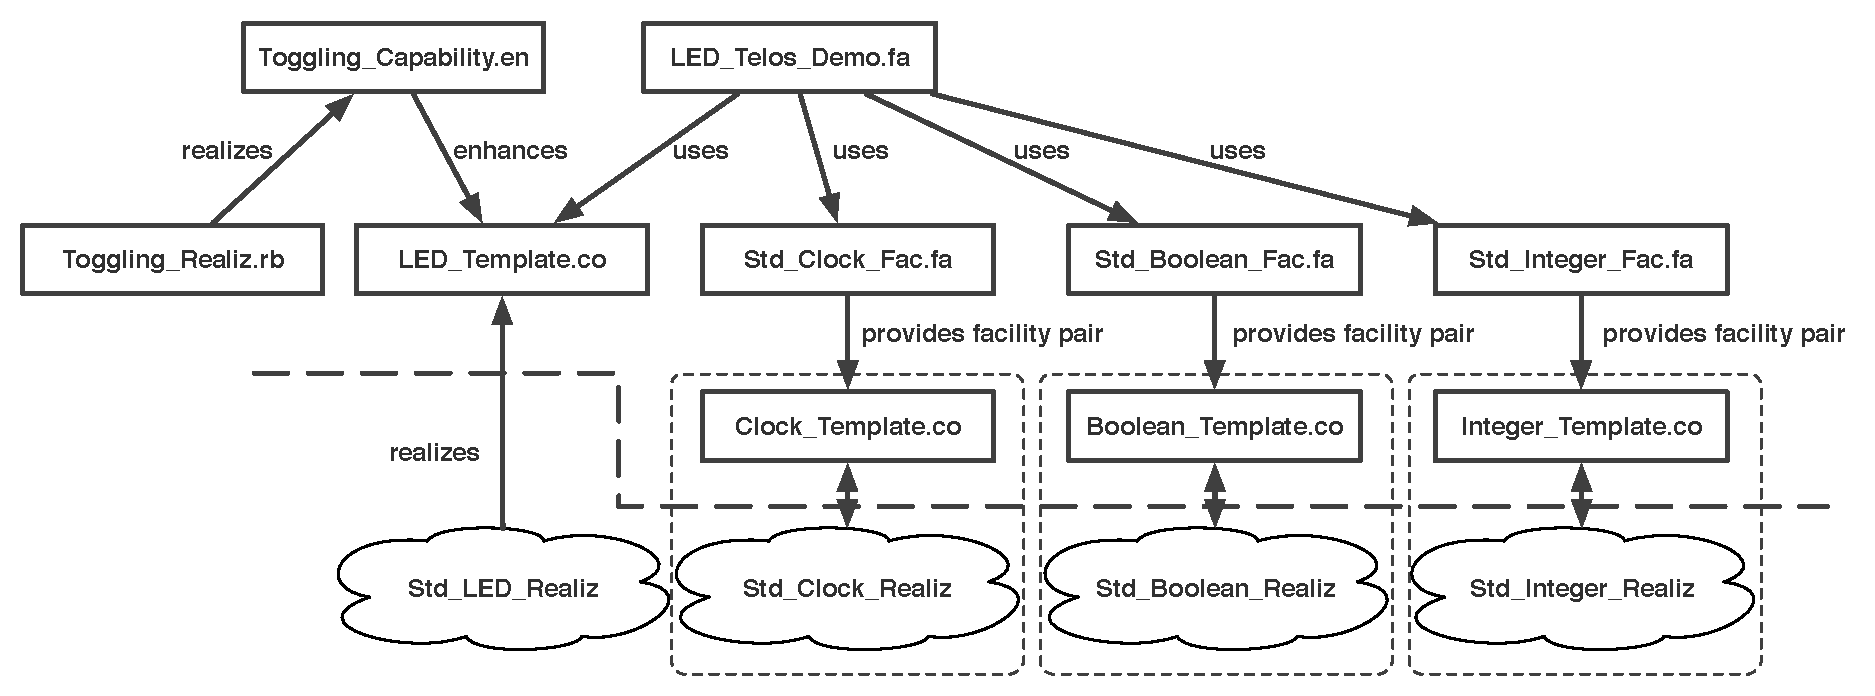
\includegraphics[scale=.55]{figs/component_graph.pdf}
\caption{A diagram illustrating inter-component relationships for the example in Section \ref{sec:specifying}}
\end{figure*}
\label{fig:imp}


Readers might note that we never presented a realization of \texttt{LED\_Template}. Indeed, after having written the concept, the RESOLVE programmer would ideally provide it with a verifiable, native RESOLVE implementation. However, as our target platform is embedded, and our concept aims to provide control for LEDs -- a decidedly low level feature on embedded hardware -- our realization is forced to operate at similarly low levels by directly manipulating hardware pins provided by msp430's chipset. 

RESOLVE, however, in its current state is too high level of a language to perform these tasks directly -- meaning it lacks the appropriate driver and language support to do so. In an effort to address this, we introduce the notion of \textit{external realizations}, which allow users to write their own realization of a concept in a language of their choosing.

The \texttt{LED\_Telos\_Demo} facility above demonstrates these developments through its use of the ``\texttt{externally realized}" phrase. This signals to the RESOLVE compiler that the user is providing a non-native realization of the \texttt{LED\_Template}, with the expectation that it conforms to the specifications dictated in the concept. 

% Applies to base types in resolve as well

% Similar to NesC, the towers of abstraction idea... eventually, similar to nesc, we get enough abstraction  through machinery such as enhancements, etc to with pieces built on top of these externally realized components.

% gives flexibility to those wishing to write other drivers and new 

We feel this new keyword is beneficial for the following reasons:
\begin{itemize}
\item The language no longer must ``hide" the fact that some of the lower level components relied upon are not written in straight-line, native RESOLVE code. The ``externally" keyword now transparently indicates this.
\item Provides flexibility for those users looking to wrap their low-level programs/drivers with formal RESOLVE interface specifications.
\end{itemize}

In the terms of embedded systems, these developments are especially as it allows us to write custom low level of the sort required for most embedded applications (e.g. LED strip drivers) while still providing formally specified interfaces that might later form the foundation . It is our hope and intention that new (native) resolve components will be layered on top of these low level, externally realized (yet specified) drivers -- eventually reaching a level of abstract where we can concern ourselves exclusively with verified, native RESOLVE components.

%In a very real sense, gives the language the capability of specifying its foundational components flexibly, and transparently which can later have all native RESOLVE components added on top. 

%More than givingHaving the freedom to use RESOLVE's specificational capabilities 

%mention performance stuff in future work section.


\begin{figure*}
\centering
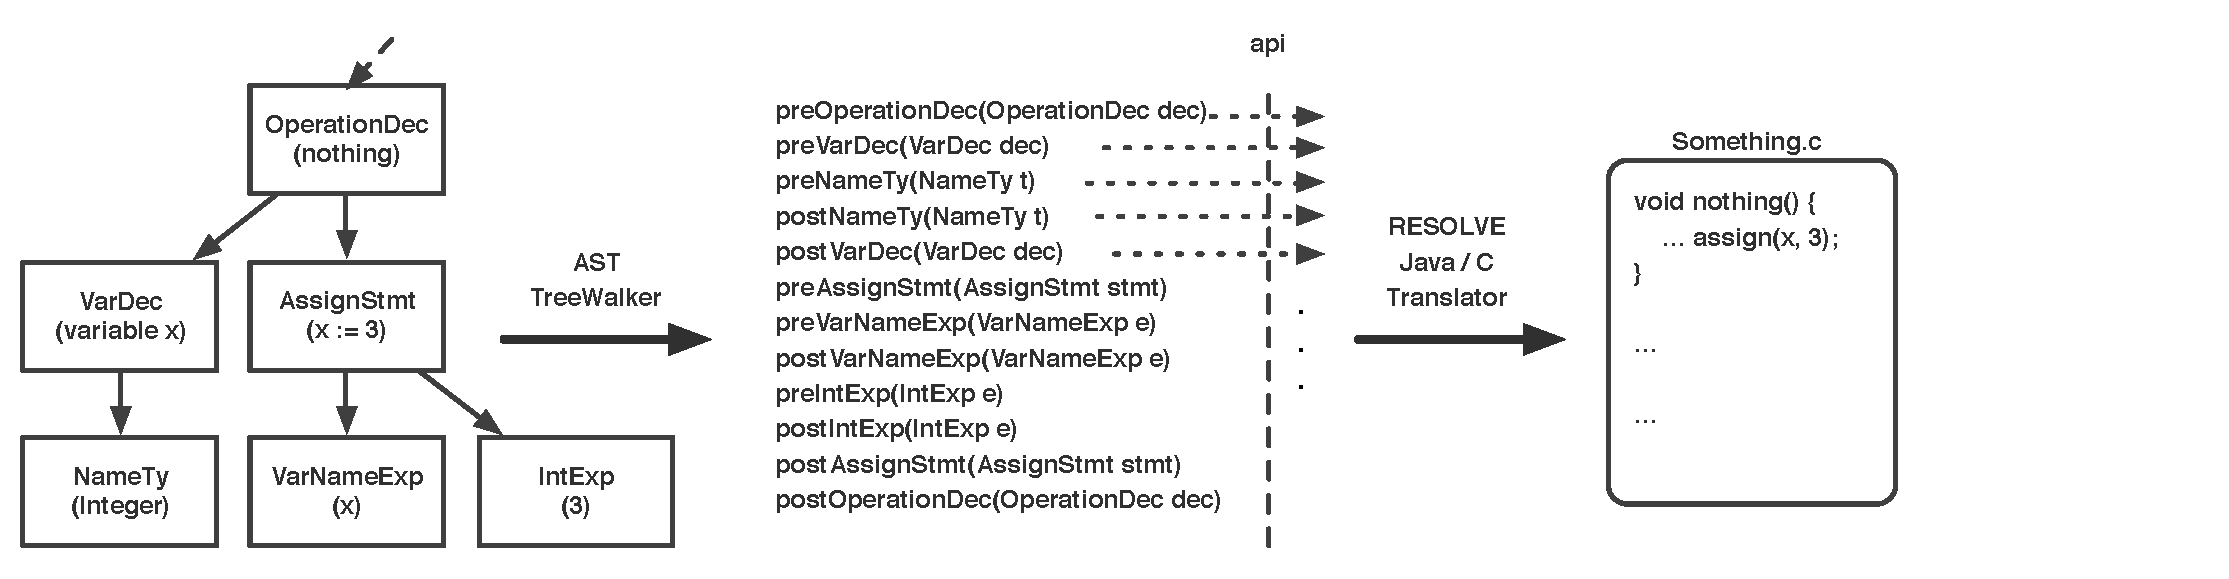
\includegraphics[scale=.55]{figs/ast_traversal.pdf}
\caption{A RESOLVE operation AST, the walk call sequence, and sample translation output.}
\end{figure*}
\label{fig:ast}
% IN THIS SECTION SHOW SOME OF OUR TRANSLATED CODE... AND WALK THROUGH IT THE SAME WAY YOU DID WITH THE CONCEPT IN RESOLVE. BUT BEFORE YOU DO THAT, SHOW THE PICTURE (The one thats already here showing high level relationships and update it!).
\section{Implementation}
Development of our C translation tool can be logically partitioned into three distinct phases: 
\begin{enumerate}
\item Arriving at a translation model (or, strategy) for an accurate C representation of RESOLVE.
\item Implementing reusable mechanisms for carrying out the C code generation process.
\item Creation of a memory manager capable of safely allocating and freeing dynamic memory required by the generated code.
\end{enumerate}
We conclude this section with a demonstration of each of these phases working in tandem on the LED component discussed in Section \ref{sec:specifiying}. 

\subsection{C Translation Model}
One of the primary challenges in translating from RESOLVE to C is finding a suitable C analog for each RESOLVE module and the constructs allowable in each. Indeed, since we are dealing with an environment where functional correctness is a primary concern, it is important that the code generated by our tool represents as closely as possible the original RESOLVE source. In an effort to make such considerations, at the highest level, the C code we generate makes special considerations for concepts, facilities, and realizations. This scheme is depicted in Figure \ref{fig:relationship} and briefly summarized in Sections \ref{sec:conceptoverview} - \ref{sec:facilitiesrealizations}.

\begin{figure}
\begin{center}
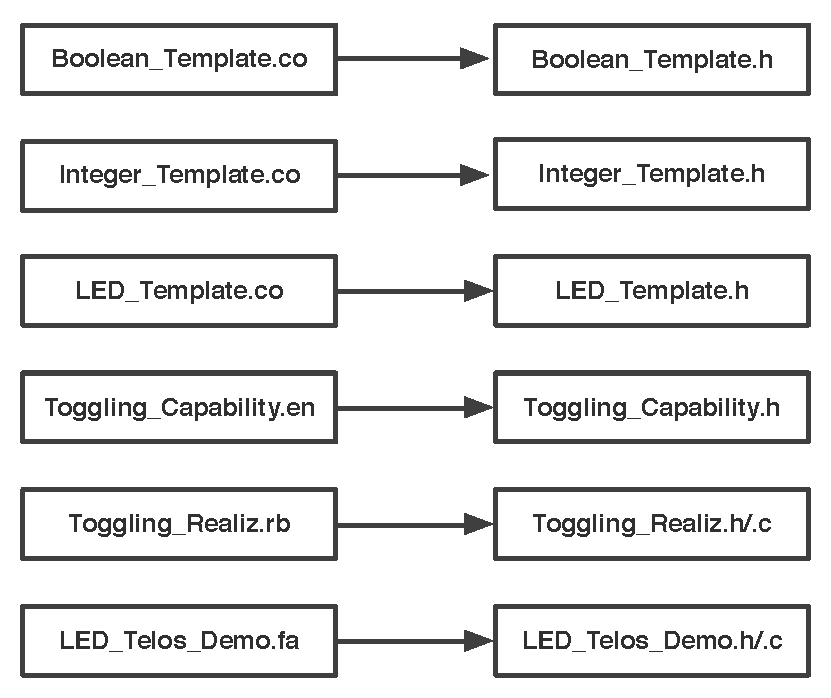
\includegraphics[scale=.60]{figs/relationship.pdf}
\end{center}
\caption{Relationship between RESOLVE module types and the C code generated from each.}
\label{fig:relationship}
\end{figure}

\subsubsection{Concepts}
\label{sec:conceptoverview}
Concept modules produce a single .h file, which provide function pointers for the operations specified in the original concept, as well as structs representing each user defined type. 

\subsubsection{Facilities}
\label{sec:facilitiesoverview}
Facilities produce an .h/.c pair: The header .h declares both a ``create" and ``destroy" method which, taken together, encapsulates the creation and destruction of all global variables used within the facility. The .c provides an implementation of these methods.  Note that these create and destroy methods are only responsible for freeing \textit{global} variables -- meaning all other translated functions are responsible for deallocating their own local variables. 

\subsubsection{Realizations}
\label{sec:facilitiesrealizations}
We treat realizations of concepts and enhancements slightly different than facility modules. While a .h/.c pair is still produced, the create method designated in the header for realizations is designed to create instances of all types specified by the concept, while the destroy method deallocates these types -- as opposed to simply destroying user created globals.

%The memory model must also be considered as an additional verifiable component. Currently, RESOLVE is not capable of creating a complete specification of memory\footnote{RESOLVE is an object based language and has variable sized structures. Using dynamically allocatable memory is the favored approach to allow arbitrarily sized data.}. Thus, a memory model must be realized without a specification. To provide a straight forward translation from RESOLVE to C, we provide a dynamically-based memory allocator for use on embedded systems.

%Unsurprisingly, concepts are represented in C by a single header .h listing the various methods 

\begin{figure*}
\begin{center}
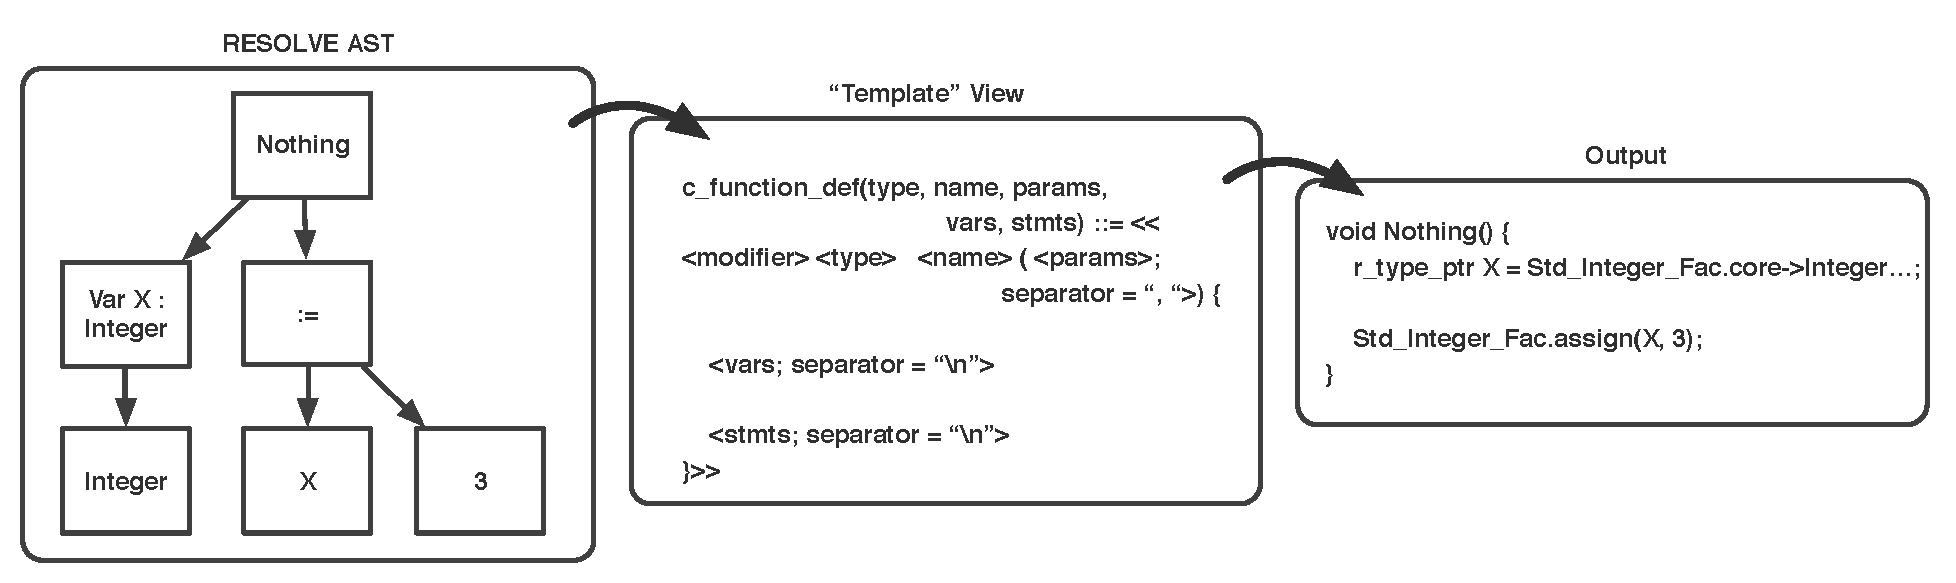
\includegraphics[scale=.55]{figs/ast_traversal2.pdf}
\end{center}
\caption{The general flow of information from the AST (first), to user defined templates (middle), ending with formed output (last).}
\label{fig:ast}
\end{figure*}


\subsection{Translator Implementation}

Translation itself occurs over the course of a traversal of RESOLVE's abstract syntax tree (AST) -- an intermediate representation of RESOLVE code. The traversal mechanism utilized is a derivative of the visitor pattern that provides a pre post traversal over all nodes in the tree. 

%\subsubsection{AST Traversal}
%Translation is performed over the course of a traversal of RESOLVE's abstract syntax tree (AST). The traversal mechanism used is a dervivative of the visitor pattern that provides a SAX-dom style pre-post traversal over all nodes in the tree. Thus, for any given node present, a total of two visits occur: One corresponding to the node being `hit' during the pre traversal stage, and one for the post. 

To illustrate the general process of producing runnable C from RESOLVE code, consider the following dummy operation:

\begin{verbatim}
Operation Nothing(); Procedure
        Var X : Integer;
        X := 3;
end Nothing;
\end{verbatim}

Shown in Figure \ref{fig:ast} is a high level depiction of steps taken in translating this operation to C. The first box depicts the AST of \texttt{Nothing}, where nodes are represented with boxes labeled by the constructs they contain. Throughout the walk of this tree, useful information (such as the operation's name, ``Nothing") are extracted from the nodes containing these constructs, and added to a user defined string-template\footnote{A template can simply be thought of as a ``document with holes" which the user choses when and how to fill.}, in this case: \texttt{c\_function\_def}.

In the context of RESOLVE to C translation, these templates, when filled during the aforementioned pre-post visitor traversal of RESOLVE's AST, help simplify the task of producing complicated, arbitrarily nested blocks of structured C output by keeping translation logic strictly within the C translator, and output logic strictly within the templates.

That is, the only actual work being performed within the C translator is forwarding information gathered from individual treenodes, to a series of externally defined templates. This allows us to exploit (in design pattern parlance) a strict model view controller (MVC) separation in the translator's codebase between the mechanism that does the AST visiting (controller), the tree nodes from which we're adding information to templates (model), and the external file containing all available C language templates which shape our output (view).

We feel this approach lends itself well to the challenge discussed in this paper, as this separation allows us to easily iterate changes to our generated C code without needing to concern ourselves with the Java written inside the compiler itself. This allows us to easily and iteratively tweak generated code -- making arbitrarily complicated changes and optimizations, some of which are detailed later in Section \#.

% general flow Each of these calls are received in the translator in the order in which they are visited within the tree. It is up to the client (in this case, the author of the C-translator) to decide which of these methods they wish to override and perform custom actions within. 

%\subsubsection{Translation output}
%Output of translated code is done using \textit{Stringtemplate} -- a third-party tool written in Java that allows users to define parameterizable templates. Like the name suggests, a template is simply ``a document with holes" that the user choses when and how to fill. 

%An example C function definition template is shown below.

%\begin{verbatim}
%function_def(modifier, type, name, params, 
%                               vars, stmts) ::= <<
%<modifier> <type> <name> (<params; sep = ", ">) {
%    <vars; sep = "\n">
%    <stmts; sep = "\n">
%}>>
%\end{verbatim}

%User supplied attributes, enclosed in \texttt{<..>}, indicates the position of that attribute relative to others. It is entirely up to the user to define which attributes to fill in, and how complex they want them to be. For example, the user might choose to fill the \texttt{params} attribute with a simple string, or a separately defined \texttt{parameter} template, which in turn might use another separately defined \texttt{type} template.

%\begin{verbatim}
%parameter(type, name) ::= "<type> <name>"
%\end{verbatim}

%In the context of language translation, these templates, when stored on a stack and manipulated over the course of the aforementioned AST traversal, help simplify the task of producing complicated, structured blocks of C output. For instance, upon visiting \texttt{preOperationDec}, a \texttt{function\_def} template can be instantiated by the client and pushed onto a global translation stack with its \texttt{name}, return \texttt{type}, and \texttt{modifier} attributes filled in. As \texttt{preOperationDec}'s children are visited, the \texttt{function\_def} template currently at the top of the stack receives similarly constructed parameter, variable, and statement templates from the nodes being walked. Upon reaching \texttt{postOperationDec}, we can be assured that the function has been completely filled in with the appropriate templates -- assuming the user has implemented the children's visit methods.

%Hence, the only actual work being performed within visit methods is forwarding appropriate information from tree-node it represents, to an externally defined template. This allows us to exploit (in shameless design pattern parlance) a strict model view controller (MVC) separation in the translator's codebase between the mechanism that does the AST visiting (controller), the tree nodes from which we're adding information to templates (model), and the external file containing all available C language templates (view).

<<<<<<< HEAD
\subsection{Memory Allocation}

Any model seeking to convert RESOLVE to a lower level representation such as C demands a strategy for handling any memory utilized by the generated code. While dynamic allocation is typically the norm, it is not however the first choice for embedded applications. With the Telos mote constrained to 128 bytes of RAM, developers targeting embedded platforms tend to favor static memory allocation over dynamic, due the memory efficiency it affords. 

%Many programs however benefit greatly from dynamic memory allocation not only in terms of clarity and straightforwardness, but in our case: Accurately modeling exactly what the code being executed is doing. 
%NesC, for example, while giving the illusion of dynamic allocation, behind the scenes actually performs static allocation 

In spite of this, our reasoning for choosing to pursue dynamic allocation over static, rests in the language itself. Being a language that relies heavily on the notion of formally specified objects (components), everything in RESOLVE from the `primitive' types such as booleans and integers, to the more complicated (user defined) ones such as Stacks and Queues, are modeled, specified, and implemented in the same way: Using the standard RESOLVE machinery discussed in Section \ref{sec:specifiying}. 

=======
%%%%%%%%%%%%%%%%%%%%%%%
%           Memory Allocation Section              %
%%%%%%%%%%%%%%%%%%%%%%%
\subsection{Memory Allocation}\label{sec:mem}

Any model seeking to convert RESOLVE to a lower level representation such as C demands a strategy for handling any memory utilized by the generated code. While dynamic allocation is typically the norm, it is not however the first choice for embedded applications. With the Telos mote constrained to 128 bytes of RAM, developers targeting embedded platforms tend to favor static memory allocation over dynamic, due the memory efficiency it affords. 

%Many programs however benefit greatly from dynamic memory allocation not only in terms of clarity and straightforwardness, but in our case: Accurately modeling exactly what the code being executed is doing. 
%NesC, for example, while giving the illusion of dynamic allocation, behind the scenes actually performs static allocation 

In spite of this, our reasoning for choosing to pursue dynamic allocation over static, rests in the language itself. Being a language that relies heavily on the notion of formally specified objects (components), everything in RESOLVE from the `primitive' types such as booleans and integers, to the more complicated (user defined) ones such as Stacks and Queues, are modeled, specified, and implemented in the same way: Using the standard RESOLVE machinery discussed in Section \ref{sec:specifiying}. 

>>>>>>> bolte
As such, even the simplest RESOLVE programs still rely heavily on the notion of objects coming and going. Thus, from a verification perspective, creating a tool that allows our translated code to create and destroy such objects in the manner the language itself uses is an important component to capture in formally verified code.

\subsubsection{Allocation using \texttt{salloc}}

<<<<<<< HEAD
The particular allocation scheme that we chose to use is \texttt{salloc()}: A first fit memory allocator. Rather than allocating memory on the heap, \texttt{salloc()} instead uses the stack. At compilation, the allocator provisions a fixed size of memory. It requires a small section of meta-data called a block which contains information of about the size of memory allocated, neighboring blocks, as well if the block is free or not. A sample representation of the stack shown in figure \ref{fig:stack}, is a typical example of allocated memory on the stack.
=======
The particular allocation scheme that we chose to use is \texttt{salloc()}: A first fit memory allocator. Rather than conventional, heap-based allocators, \texttt{salloc()} uses stack memory for allocation. This approach requires that a fixed size of memory is chosen at compilation. In addition, \texttt{salloc()}, requires a section of meta-data, which is denoted as a \texttt{block}, for each record in the memory pool. A \texttt{block} holds referential information of neighboring blocks, the size of the record the block maintains, and if the block is free or is in use. Figure~\ref{fig:stack} is an example of the stack after several calls to \texttt{salloc()}.
>>>>>>> bolte

\begin{figure}[!htb]
%\centering
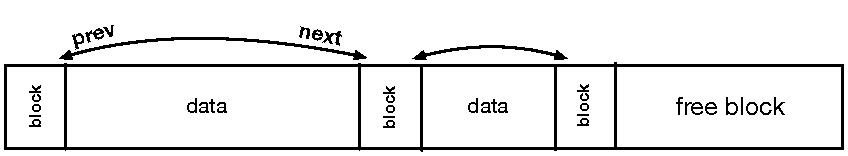
\includegraphics[scale=.55]{figs/stack.pdf}
\caption{Representation of memory using salloc()}
Memory allocated with salloc() allocates a block in front of data allocated. Blocks point to their immediate neighbors and hold their size and usage.
\label{fig:stack}
\end{figure}

\subsubsection{Deallocation using \texttt{sfree}}

A memory allocator must provide a mechanism to release, or free memory in order to indicate that it is not being used and can be reallocated. The \texttt{sfree()} function provides deallocation for memory allocated with \texttt{salloc()}. Figure~\ref{fig:free} shows an example set of memory before and after calling \texttt{sfree()}. 

\begin{figure}[!htb]
%\centering
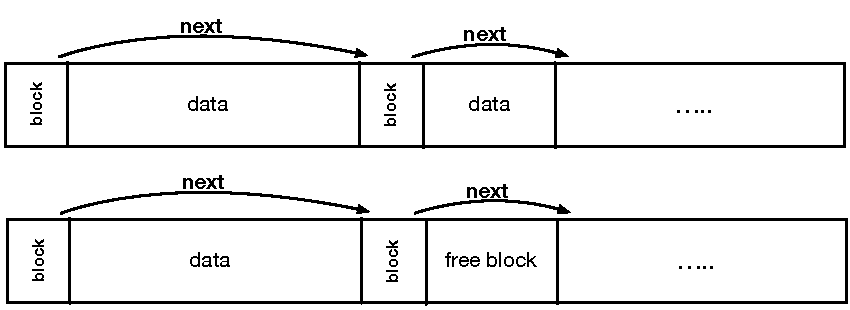
\includegraphics[scale=.55]{figs/sfree.pdf}
\caption{sfree to free memory}
\label{fig:free}
\end{figure}

\subsubsection{Optimizing Memory Usage}

A common problem that can occur in memory allocation is fragmentation. During execution, a program can allocate and deallocate an arbitrary number of times. Figure~\ref{fig:fragmentation} shows problems that result from this. This problem is magnified on embedded systems due to their limited memory capacities. There are simple optimizations that can reduce fragmentation. 

Block splitting, as shown in Figure~\ref{fig:split}, occurs during allocation. It allows blocks of greater size to be partitioned into the size requested by the allocator. 

Fusing blocks is another technique used when \texttt{sfree()} is called. When memory is deallocated, neighboring free blocks are coalesced to form a single large block, as shown in Figure~\ref{fig:fuse}. 

\begin{figure}[!htb]
\centering
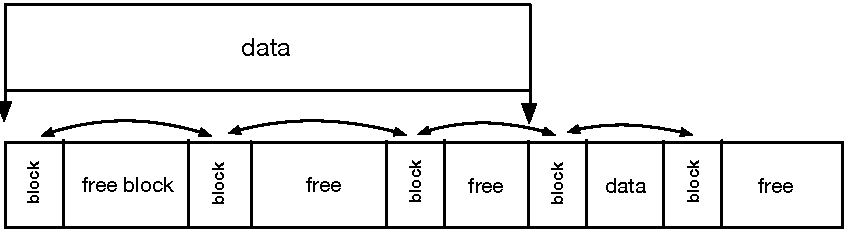
\includegraphics[scale=.55]{figs/fragmentation.pdf}
\caption{Performing naive allocation and deallocations, allocatable blocks are restricted to those that match the exact size of memory requested from the allocator}
\label{fig:fragmentation}
\end{figure}

\begin{figure}[!htb]
\centering
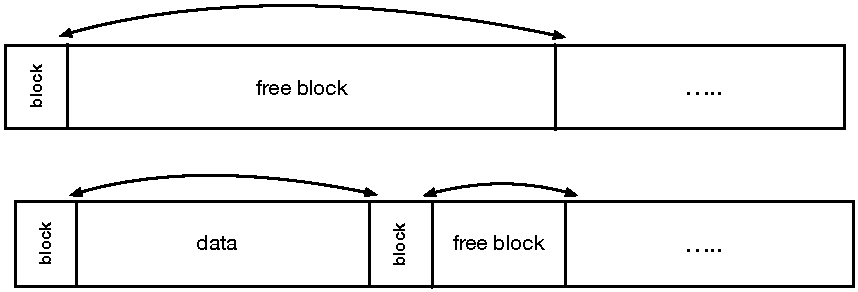
\includegraphics[scale=.55]{figs/split.pdf}
\caption{Splitting creates a block that is the size that the allocator requested, and a new free block with the remainder of memory.}
\label{fig:split}
\end{figure}


\begin{figure}[!htb]
\centering
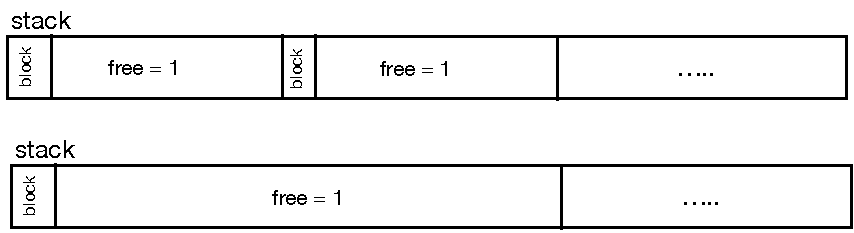
\includegraphics[scale=.55]{figs/fuse.pdf}
\caption{Block fusing. This creates single larger block, decreasing the number of smaller blocks unable to split.}
\label{fig:fuse}
\end{figure}

%
%

% An LED Demo Translation
\section{LED Demo}

\begin{figure*}
\begin{minipage}{0.4\textwidth}
\begin{verbatim}
/*
 * Generated by the RESOLVE to C translator. 
 * This file should not be modified.
 */
#ifndef __LED_TELOS_DEMO_H
#define __LED_TELOS_DEMO_H

#include ".../RESOLVE.h"
#include ".../Facilities/.../Std_Bool_Fac.h"
#include ".../Facilities/.../Std_Int_Fac.h"
#include ".../Facilities/.../Std_Clock_Fac.h"
#include ".../Concepts/.../LED_Template.h"
#include ".../Concepts/.../Std_LED_Realiz.h"
#include ".../Concepts/.../Toggling_Realiz.h"

typedef struct LED_Facility LED_Facility;
struct LED_Facility {
    LED_Template* core;
    Toggling_Capability_for_LED_Template* 
                      Toggling_Capability;
};
LED_Facility LED_Fac_Var;

void LED_Telos_Demo_create();
void LED_Telos_Demo_destroy();
#endif
\end{verbatim}
\end{minipage}
\hspace{1.5cm} 
\begin{minipage}{0.4\textwidth}
\begin{verbatim}
/*
 * Generated by the RESOLVE to C translator. 
 * This file should not be modified.
 */
#include "LED_Telos_Demo.h"

void LED_Telos_Demo_create() {
  Std_Bool_Fac_create();
  Std_Int_Fac_create();
  Std_Clock_Fac_create();
  r_type_ptr __arg_0 = Std_Int_Fac_Var.core->
    createFromInt(4, Std_Int_Fac_Var.core->Integer);
  LED_Fac_Var.core = 
    new_Std_LED_Realiz_for_LED_Template(__arg_0);
  LED_Fac_Var.Toggling_Capability = 
    new_Toggling_Realiz_for_
    Toggling_Capability_of_LED_
    Template(LED_Fac_Var.core);
  Std_Int_Fac_Var.core->Integer->
    destroy(__arg_0, Std_Int_Fac_Var.core->Integer);
}

void LED_Telos_Demo_destroy() {
    free_Std_LED_Realiz_for_LED_Template(
    				    LED_Fac_Var.core);
    Std_Bool_Fac_destroy();
    Std_Int_Fac_destroy();
}
        ...
\end{verbatim}
\end{minipage}
\end{figure*}



\section{Related Work}

Though RESOLVE is the only system we know of that proves, prior to compilation, the full functional correctness of embedded software, there are a number of other systems that 
%There are a number of existing systems that ultimately seek to prove the functional correctness of programs. While we discuss only two here, readers interested in learning more about the systems mentioned might to refer to \cite{klebanov:2011} for a more in depth discussion. Perhaps most notable among the systems we list here (and perhaps the closest to RESOLVE's approach) is Microsoft research's Dafny \cite{leino:2010}. Designed to be capable of verifying pointer based structures, Dafny currently stands as one of the more popular approaches to verification. Substituting RESOLVE's notion of mathematical variables with what are termed `ghost' variables, reasoning is kept, like RESOLVE, disconnected from implementation-level code. Dafny uses an intermediate verification language, termed Boogie, to generate verification conditions which are then dispatched via Z3, Microsoft's automated prover. 

%Another system, also a Microsoft research endeavor, is VCC -- a system designed for the verification of C programs \cite{vcc:2009}. One of the main draws of VCC is that it has mechanisms for verification of concurrent code -- an ideal feature when presented with asynchronous, event driven code common in most embedded applications. 

%RESOLVE differs from the projects mentioned above most notably in that it does not make use of third party automated provers or decision procedures to discharge verification conditions. Rather, it makes use of an integrated, minimalist term rewrite prover that applies higher order theorems and definitions in attempting to transform givens into a provable goal. 

% shortcoming -- concurrency.

\section{Discussion and Future Work}

Using embedded application development as an example, we perceive this work as a step towards more fully exploring the role of formal verification in lower level system-oriented contexts. Indeed, the realm of embedded systems provides an ideal stepping off point for this challenge, as it encourages (and indeed, requires) RESOLVE to provide support for not only new target languages (namely C), but also new language constructs that give the user the ability to author drivers required for any serious embedded application. While we have made progress with the latter in the form of the externally keyword, a natural direction for future work would entail using RESOLVE's performance specification mechanisms to prove the time and duration estimates for a memory allocator, not unlike the one presented here. Indeed, by being able to prove aspects of this system at this level of granularity (down to time and space) confidence in the systems we rely upon everyday (embedded systems included) 

proving memory and time constraints on any allocation scheme will provide assurance that we never exceed limitations or behave unexpectedly.

Moreover, if we do In the future if we do it dynamically or statically there is no difference, if the static people are concerned about memory, the It might not seem like we're doing much w

Further, an additional language characteristic that we feel would be beneficial is having some means of dictating \textit{static objects}. While RESOLVE makes considerations for single instance concepts that are tied to particular facility instantiations, we currently have no means of strictly limiting how many instantiations of a particular facility there might be (not even via standard facilities). Thus, in terms of specifying concepts such as clocks, LED strips, and other hardware-centric concepts that only appear once on a circuit board, RESOLVE could benefit from a mechanism that restricts allowable instances of these and other objects. 

\section{Conclusion}

In this paper we present a new RESOLVE language construct, and a translation tool that aims to produce an accurate, embedded platform-friendly C representation of RESOLVE. We provide representative specifications of an LED strip component that both demonstrates the benefits of RESOLVE's approach to reusable mathematical developments, as well as formal verification of a single driver enhancement. We illustrate usage of this component in the context of a client facility module, wherein we introduce the externally keyword that allows users to transparently pair non-native RESOLVE implementations with native RESOLVE specifications. We then translate this facility application, illustrating a proof-of-concept dynamic memory allocator working in tandem with what we consider to be an accurate C representation of RESOLVE code. The examples and results listed in this paper have been successfully run on a Telosb mote, and the overall tool -- now fully integrated with the RESOLVE compiler -- actively continues to undergo improvements and optimizations on all fronts.

\section{Acknowledgements}

Special thanks to Mike Kabanni, Mark Todd, and Bruce Weide whose suggestions and initial contributions in constructing the current model of RESOLVE to C translation made this work possible. 

%Open up the .tex file and compile it using Latex (Shift+Apple+L) then compile it using Bibtex (Shift+Apple+B)
\bibliographystyle{unsrt}
\bibliography{sigproc}
\end{document}